\chapter{User Guide} \label{chap:b}
The purpose of this chapter is to provide a user guide on how to use the software proposed in this article. Each section provides instructions for different subcomponents of the framework. Note that the required python modules must be installed before running any of the software. They can be found in the software/python\_libraries/requirements.txt file. These dependencies can be installed by creating a virtual environment at the root of this project and running the command:
\begin{figure} [h]
    \centering
    $pip3$ $install$ $-r$ $requirements.txt$
\end{figure}

Please note that most directories also contain README.md files with instructions and descriptions for using the software.

\section{How to generate scenarios} \label{sect:b.1}
This section gives a brief overview of how to generate the scenarios. The scenario generation script can be found in the software/generating\_scenarios directory and is named \textbf{create\_scenario.py}. It takes the following optional arguments:

\begin{itemize}
  \item -d the difficulty of the scenario ($0 \leq d \leq 1000$)
  \item -s the sun altitude ($-90 \leq s \leq 90$), where 90 means that the sun is at its peak and -90 means that it is an absolute night
  \item -w the weather wetness level in the scenario ($0 \leq w \leq 100$)
  \item -f the name of the file to save the scenario to (without the .json ending)
  \item -r flag meaning that the algorithm should be trained using a randomisation seed (the same every time)
\end{itemize}

An example of the command in the terminal can be seen in the image below:

\begin{figure} [h]
    \centering
    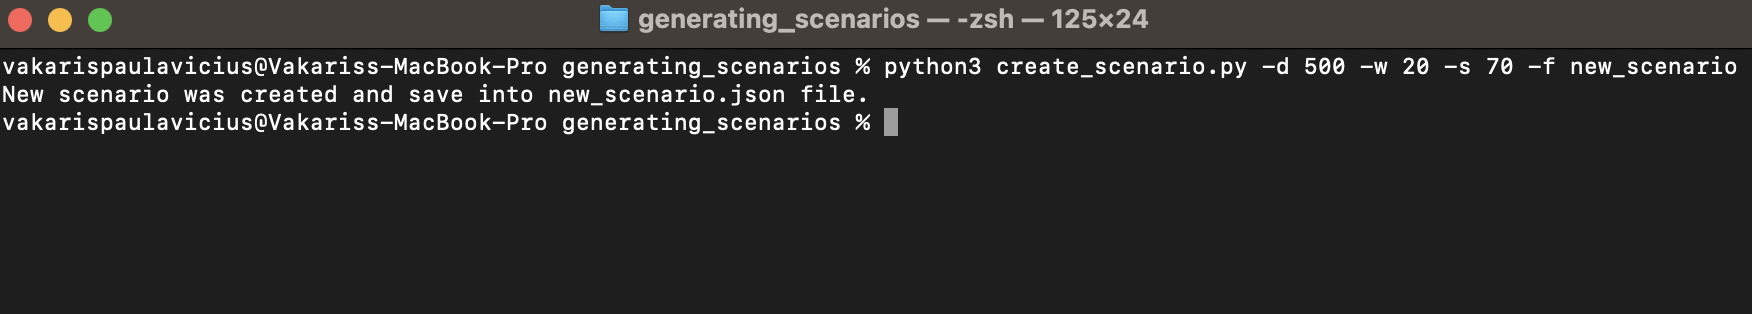
\includegraphics[width = 0.9\textwidth]{research_paper/Images/create_scenario.png}
    \caption{How to generate a scenario}
\end{figure}

The following command would generate a new scenario in a new file \textbf{new\_scenario.json} and save the file to the data/scenario\_generation\_data/generated\_scenarios directory. The file can be later used to create a specific path, or it could be used as a predefined scenario for the simulations.

\section{How to build paths} \label{sect:b.2}
This section briefly overviews how a script that builds paths can be run. The script itself is located in the software/carla\_scripts directory. Its name is \textbf{path\_generator.py}. It takes the following mandatory arguments:
\begin{itemize}
  \item -f the name of the file to save the built path to (without the .json ending)
  \item -s the name of the scenario to be referenced when designing the path (without the .json ending)
\end{itemize}

An example of the command in the terminal can be seen in the image below:

\begin{figure} [h]
    \centering
    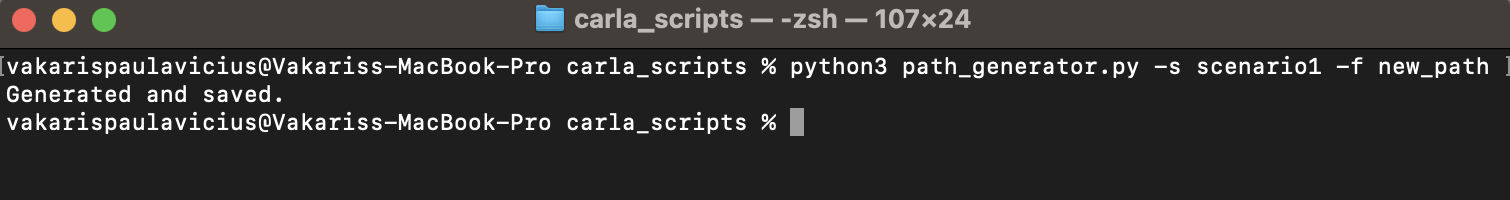
\includegraphics[width = 0.9\textwidth]{research_paper/Images/build_path.png}
    \caption{How to build a path}
\end{figure}

The following command would build a new path in the file \textbf{new\_path.json} and save the file to the data/paths directory. The file can be later used as a predefined path for scenarios or inspected on the map using helper scripts, for instance, draw\_lanes\_terminal.py.

\section{How to run the simulations} \label{sect:b.3}

This section presents a simple way of running the scenarios. At first, the user has to decide how many scenarios he wants the software to run and whether the scenarios should be predefined or created at run-time. If the user decides to use predefined scenarios, he must describe that in the scenario\_list.json file in the software/carla\_scripts directory. An example of the scenario list can be seen in \autoref{fig:scenario_list}. If the user wants the path and the scenario to be generated at run-time, the attributes "name" and "details" of each scenario element in the scenario list file should be set to $null$. The scenario simulation process requires the CARLA simulator to be running. Once the CARLA simulator is running and accessible, the user needs to navigate to the software/carla\_scripts directory in the second terminal and run the following command to run the simulations with manual control:

\begin{figure} [h]
\centering
        $/run.sh$ $[name]$
\end{figure}
In order to change whether the steering wheel is to be used or the keyboard, the user needs to comment and uncomment lines 157 and 158 in scenario\_manager.py, respectively. 

The element [name] needs to be replaced by the name given to the participant. All the recorded data will be stored in the data/recordings/[name] directory, and the details of the simulations will be visible in the data/recordings/[name]/session\_logs.log file. In order to launch the Carla agent, the following command has to be run:

\begin{figure} [h]
    \centering
    $/run.sh$ $[name]$ $ai$
\end{figure}

The keyword "ai" (at the end of the line) differentiates manually controlled and self-driving cars. \textbf{Important: if at any point the program crashes and the cause is unknown, the parts "$>$ /dev/null 2 $>$ \&1" need to be commented out on lines 26 and 33 in the run.sh script in addition to line 160 in the scenario\_manager.py script. This allows for message output to the terminal.} All the errors should be handled by the try-except blocks, and the appropriate messages should be written to the session\_logs.log files. The steps mentioned before work as a plan b if something goes wrong.

\section{How to perform analysis} \label{sect:b.4}
Two types of analysis can be performed. Let us start with the analysis method meant to assist in the score calculation process called scenario analysis. The script can be found in the software/data\_analysis directory and is called scenario\_analyser.py. It aims to analyse both the scenario and the path and extract information such as the average allowed speed on the path, the number of pedestrian crossings and other. Note that in order to run this script, the CARLA simulator must be running. This is needed because the script needs to use the built-in functions of CARLA and access the map attributes. The script takes two mandatory arguments:

\begin{itemize}
  \item -p the name of the path (without the .json ending)
  \item -s the name of the scenario (without the .json ending)
\end{itemize}

The following command is used to perform the scenario analysis:

\begin{figure} [h]
    \centering
    $python3$ $scenario\_analyser.py$ $-s$ $scenario1$ $-p$ $path1$
\end{figure}

As a result, it produces a file named the same as the scenario given as the argument. It saves this file into the data/simulation\_details directory. This file is later used by the score calculator discussed in \autoref{sect:b.6}

The second analysis tool is responsible for analysing the recordings of the scenario runs. It synthesises and processes information that is later used by the visualisation tools. The data analysis tool can be found in the software/data\_analysis directory and is named \textbf{run\_analysis.sh}. It takes a name as an argument and processes the recordings according to the specifications in the analysis\_parameters.json file. How the parameters file looks can be seen in \autoref{fig:analysis_parameters}. It creates a new directory in data/analysed\_data/data with the name provided as the argument and stores the analysed data there. 

The following command can be used to run an example analysis:

\begin{figure} [h]
    \centering
    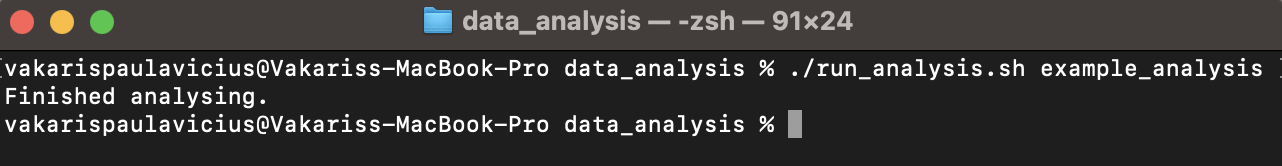
\includegraphics[width = 0.9\textwidth]{research_paper/Images/data_analysis_how_to.png}
    \caption{How to perform data analysis}
\end{figure}

\section{How to draw diagrams and maps} \label{sect:b.5}
This section discusses how to visualise the analysed data. The visualisations can be done in two ways: drawing the diagrams or visualising interesting points on the map. Let us look at the diagram drawing first. The diagram drawing script can be found in the software/data\_analysis/visualisation/diagram\_drawing directory. In order to make matters easier, an example file is provided in the directory, and it is called draw\_diagram\_example.sh. The comments in the script show which places should be edited to draw different diagrams. More about the customisations of it was discussed in \autoref{sect-7.2} when we talked about how the visualisation of data is performed. The following command would produce an image from \autoref{fig:diagram_example}.

\begin{figure} [h]
    \centering
    $./draw\_diagram\_example.sh$
\end{figure}

For the map visualisation, the crdesgner module is required. If all the modules from the requirements.txt file were installed successfully, as mentioned at the beginning of this chapter, then it should already be present in the system. However, this project modified the module to better fit the project's needs. In order to perform the map visualisation, the modified version from software/python\_libraries/crdesigner needs to be used. Simply replace the package in the system with the one provided in this project's repository.

As with the diagram drawing, an example script is provided in the software/data\_analysis/vi-
sualisation/map\_drawing directory. Its name is draw\_map\_example.sh. In order to draw a different map or a different list of points, the script's code should be edited accordingly. The following command should produce a view similar to the one in \autoref{fig:map_drawing}.

\begin{figure} [h]
    \centering
    $./draw\_map\_example.sh$
\end{figure}

Note that if maps other than the ones provided by CARLA are used in the simulations, their OpenDRIVE description files must be added to the data/maps/opendrive\_format directory. For the CommonRoad Scenario Designer to depict them, they must be converted from OpenDRIVE to CommonRoad format. It is done by the xml\_converter.py script present in the data/maps directory.


\section{How to calculate the score} \label{sect:b.6}
This section concludes the user guide by examining how the participant's performance in a specific scenario can be evaluated. It is done by the score\_calculator.py script present in the software/data\_analysis directory. The script takes two mandatory arguments:

\begin{itemize}
  \item -n the name of the participant
  \item -s the name of the scenario (without the .json ending)
\end{itemize}

It then looks at the files in data/recordings/[participant's name]/[scenario], extracts the necessary information and calculates the score printing it to the terminal. The following is an example of how this is done:

\begin{figure} [h]
    \centering
    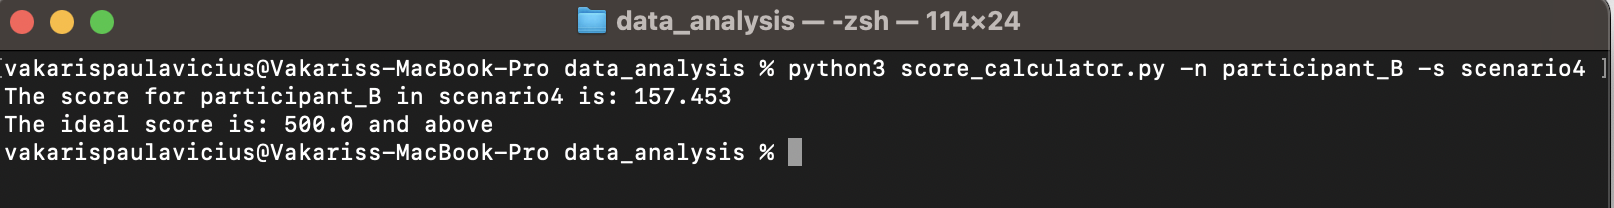
\includegraphics[width = 0.9\textwidth]{research_paper/Images/score_calculation.png}
    \caption{How to evaluate the performance}
\end{figure}

In addition to calculating the score and printing it to the terminal, the script also provides the ideal score for that particular scenario. The scores are calculated based on the formula introduced in \autoref{sect-6.3}.
